
%(BEGIN_QUESTION)
% Copyright 2010, Tony R. Kuphaldt, released under the Creative Commons Attribution License (v 1.0)
% This means you may do almost anything with this work of mine, so long as you give me proper credit

Decode the following serial data streams, each one encoded using a different method:

$$
\includegraphics[width=15.5cm]{i02917x02.eps}$$

\vskip 30pt

$$\includegraphics[width=15.5cm]{i02917x03.eps}$$

\vfil 

\underbar{file i02917}
\eject
%(END_QUESTION)





%(BEGIN_ANSWER)

This is a graded question -- no answers or hints given!

%(END_ANSWER)





%(BEGIN_NOTES)

Recall that each rising edge on a clock pulse is a ``1'' while each falling edge on a clock pulse is a ``0''.  The only real challenge after this is identifying which transitions coincide with clock pulses and which transitions are merely ``reversals'' setting up for the next real bit.  Here, spacing is key: every pair of transitions separated by a wide time interval must be real bits.  Once you identify any two data bits, you may measure the spacing of those bits up and down the rest of the waveform to identify the data bits and to ignore the reversals:

$$\includegraphics[width=15.5cm]{i02917x01.eps}$$

\vskip 10pt

FSK encoding is relatively simple: each high-frequency burst is a ``0'' while each low-frequency burst is a ``1'':

$$\includegraphics[width=15.5cm]{i02917x04.eps}$$

In both cases, and indeed with {\it all} serial data formats, it is important to note that the data bits will occur at regular intervals, because they follow a fixed clock cycle.

%INDEX% Electronics review: Manchester encoding
%INDEX% Electronics review: FSK encoding

%(END_NOTES)

